
\section{Minimal surfaces and persistent homology} \label{s:surfaces}

Having established Morse inequalities in terms of persistence diagrams and topological conditions for existence of persistence diagrams associated to filtrations, we now connect these results to the work of Morse and Tompkins on minimal surfaces from \cite{Morse.1939}.
We will focus on the homological aspects of their approach.
For a general exposition we refer to \cite[Sections 4.3--5]{Bott.1980}, and for a more detailed exposition including the analytical details see \cite[Section II.6]{Struwe.1988}.

Morse and Tompkins considered the following setting introduced by Douglas.
Let $g \colon \R \to \R^n$ be a $2\pi$-periodic function representing a simple closed curve such that $g$ is differentiable with Lipschitz derivative.
Let $\widetilde{\Omega}$ be the space of continuous functions $\varphi \colon \R \to \R$ with $\varphi((t)+2\pi) = \varphi(t) + 2\pi$ for all $t$ and such that there are three distinct points $\alpha_i \in [0,2\pi)$ with $\varphi(\alpha_i)=\alpha_i$.
The \emph{Douglas functional} on $\widetilde \Omega$ associated to the curve $g$ is defined by
\begin{equation*}
A_g(\varphi) = \frac{1}{16} \int_0^{2\pi} \int_0^{2\pi} \sin \left( \frac{\alpha-\beta}{2} \right)^{-2} \! \lVert g(\varphi(\alpha)) - g(\varphi(\beta)) \rVert_2^2 \ \mathrm{d}\alpha \ \mathrm{d}\beta.
\end{equation*}
Let $\Omega_g = \{\varphi \in \widetilde\Omega \mid A_g(\varphi) < \infty\}$.
Douglas proved that, for a large class of curves $g$, the set $\Omega_g$ is non-empty and the sublevel sets of $A_g$ are compact.
Since $A_g$ is bounded below by $0$, this implies that $A_g$ has a unique global minimizer.
Using methods from harmonic analysis, Douglas then showed that this minimizing critical point of $A_g$ corresponds to a solution of Plateau's Problem.

As alluded to in \cref{r:homotopically critial points}, Morse and Tompkins consider a homotopical notion of critical point for a general function $F \colon M \to \R$ on a metric space \cite[p.~445]{Morse.1939}, see also \cite{Morse.1943}.
Roughly, a point $p$ is \emph{homotopically critical} if it has no neighborhood in $M_{\leq F(p)}$ that can be mapped by a homotopy into $M_{\leq t}$ for some $t<F(p)$.

Morse and Tompkins prove that each homotopically critical point of the functional $A_g$ corresponds to a critical point of the area functional, called a minimal surface, and use this correspondence to prove the following result \cite[p.~447]{Morse.1939}, also reviewed as Theorem II.6.10 in \cite{Struwe.1988}.

\begin{thm}[Unstable Minimal Surface Theorem]
	If $\Omega_g$ contains two distinct solutions to Plateau's Problem then it also contains an unstable minimal surface, more precisely, a critical point of $A_g$ of index 1.
\end{thm}

Their proof relies on Morse inequalities for homotopically critical points, which they infer by relating these critical points to the cap numbers associated to the persistent \v{C}ech homology of the sublevel set filtration of the function, and then applying the Morse inequalities for cap numbers as we have considered them in \cref{s:inequalities}, and as Morse considered them in \cite{Morse.1940}.

We have seen that these inequalities require q-tameness, so in order to apply them and deduce their theorem, Morse and Tompkins need to prove the \mbox{q-tameness} of $(\Omega_g, A_g)$.
Throughout his work on functional topology, in order to obtain \mbox{q-tameness}, Morse assumed slightly varying forms of local connectivity on the resulting sublevel set filtrations.
In particular, in their applications to minimal surface theory, Morse and Tompkins used the following condition:
\begin{displaycquote}[p.~431]{Morse.1940}
	The space $M$ is said to be \emph{locally $F$-connected} of order $r$ at $p$ if corresponding to each positive constant $e$ there exists a positive constant $\delta$ such that each singular $r$-sphere on the $\delta$-neighborhood of $p$ on $F_{c+\delta}$ bounds an $(r+1)$-cell of norm $e$ on $F_{c+e}$.
\end{displaycquote}
Here, $c = F(p)$.
Using similar language to the one used in \cref{s:connectivity}, this property is equivalent to the following notion applicable to general topological spaces.

\begin{defi}
	The sublevel set filtration of a function $f \colon M \to \R$ is said to be \emph{weakly homotopically locally connected} or \emph{weakly $\piLC$}	if for any $x \in X$, $V$ a neighborhood of $x$, and any index $t > f(x)$, there is an index $s$ with $f(x) < s < t$ and a neighborhood $U$ of $x$ with $U \subseteq V$ such that the inclusion $f_{\leq s} \cap U \to f_{\leq t} \cap V$ induces trivial maps on homotopy groups.
\end{defi}

Morse then goes on to state that as a consequence of local $F$-connectivity the persistent \v{C}ech homology of this sublevel set filtration is q-tame.
In the original it reads:
\begin{displaycquote}[Theorem 6.3, p.~432]{Morse.1940}
	Let $a$ and $c$ be positive constants such that $a < c < 1$.
	The $k^{\mathrm{th}}$ connectivity $R^k(a,c)$ of $F_a$ on $F_c$ is finite.
\end{displaycquote}
Morse does not prove this statement in the given reference, but rather refers to \cite[Theorem~6.1]{Morse.1938}.
Unfortunately, the above claim does not hold in general, as we will show next by providing an explicit counterexample.

\begin{defi}
	The sublevel set filtration of a function $f \colon X \to \R$ is said to be \emph{weakly locally connected} or $\LC$ if for any $x \in X$, $V$ a neighborhood of $x$, and any index $t > f(x)$, there is an index $s$ with $f(x) < s < t$ and a neighborhood $U$ of $x$ with $U \subseteq V$ such that the inclusion $f_{\leq s} \cap U \to f_{\leq t} \cap V$ is homotopic to a constant map.
\end{defi}

Clearly, being weakly $\LC$ implies being weakly $\piLC$ and, if the homology $\H$ takes finite dimensional values on one point spaces, also weakly $\HLC$.
We will now show that not even weakly $\LC$ is sufficient to ensure the q-tameness of compact sublevel set filtrations that are induced by non-continuous functions.
In particular, our construction will be used to invalidate Morse's claim quoted above.

We will consider the \emph{$d$-dimensional Hawaiian earring}
\begin{equation*}
\HE = \bigcup_{n \in \N} \left\{ (x_0, \dots, x_d) \in \R^{d+1} \ \middle | \ \left( x_0 - \frac{1}{n} \right)^2 \!\! + x_1^2 + \dots + x_d^2 = \left( \frac{1}{n} \right)^2 \right\},
\end{equation*}
which is a compact subspace of $\R^{d+1}$.

\begin{figure}[t]
	\centering
	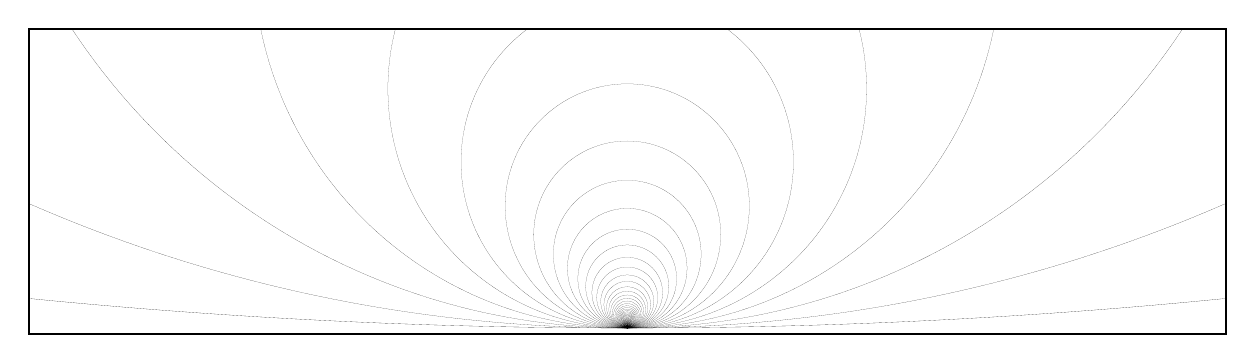
\begin{tikzpicture}[scale = 76]
	\draw[thick] (-.1,-.001) rectangle (.1,.05);
	\clip (-.1,0) rectangle (.1,.05);
	\foreach \i in {1,...,100}{
		\draw[line width=0.1/\i mm] (0, 1/\i^2) circle (1/\i^2);
	}
	\end{tikzpicture}
	\caption{A closeup of the Hawaiian earring $\mathbb{H}^1$.}
\end{figure}

\begin{thm} \label{t:counterexample}
	The function $f \colon \HE \to \R$ whose value at the origin is $0$ and is $1$ everywhere else defines a compact and weakly $\LC$ sublevel set filtration that is not q-tame with respect to $\H$ if $\H_{n}(\HE)$ is infinite dimensional for some $n$.
\end{thm}

\begin{proof}
	To verify that $f$ has compact sublevel sets we notice that all sublevel sets are either the empty set, the singleton containing the origin, or $\HE$ itself, all compact Hausdorff spaces.
	
	In order to verify that the sublevel set filtration of $f$ is weakly $\LC$, we
	consider $x \in \HE$, $V$ a neighborhood of $x$ in $\HE$ and $t > f(x)$. We need to find a neighborhood $U \subseteq V$ of $x$ and $s \in (f(x), t)$ such that the inclusion $f_{\leq s} \cap U \to f_{\leq t} \cap V$ is homotopic to a constant map.
	
	If $x$ is the origin, we have $f(x) = 0$ and choose $s \in (0, \min\{t, 1\})$.
	Then $f_{\leq s} = \{x\}$, so with $U = V$ the inclusion $f_{\leq s} \cap U \to f_{\leq t} \cap V$ is the inclusion of $\{x\}$ into $f_{\leq t} \cap V$, which is a constant map, so the weak $\LC$ condition is trivially satisfied.
	
	For $x$ not the origin we have $f(x) = 1$ and choose $s \in (1,t)$ arbitrarily, so that $f_{\leq s} = f_{\leq t} = \HE$. 
	Note that since $x$ is not the origin, there is a unique $d$-sphere in $\HE$ that contains $x$.
	Clearly, we may choose $\delta > 0$ so small that $D_{\delta}(x) = \{y \in \R^{d+1} \mid \Vert x - y \Vert < \delta\} \cap \HE$ is a topological disk contained in this sphere and contained in $V$. 
	The disk $D_\delta(x)$ can be contracted to $\{x\}$ in $V$, so choosing $U = D_{\delta}(x)$, we obtain that the inclusion $f_{\leq s} \cap U \to f_{\leq t} \cap V$ is homotopic to the constant map with value $x$.
	
	It remains to be shown that $f_{\leq \bullet}$ is not q-tame for $\H$.
	This follows directly from our assumption that $\H_{n}(\HE)$ is not finite dimensional for some $n$, as $f_{\leq t}$ is constant with value $\HE$ for $t \geq 1$.
\end{proof}
\newpage
Both singular and \v{C}ech homology of the $d$-dimensional Hawaiian earring is infinite dimensional in degree $d$, so they satisfy the assumptions of \cref{t:counterexample}.
For singular homology this is proven in \cite{Barratt.1962}.
For \v{C}ech homology, one can use the fact that it commutes with totally ordered limits for compact Hausdorff spaces \cite[Theorems VIII.3.6.\@ and X.3.1.]{Eilenberg.1952} as follows.
Define 
\begin{align*}
\HE_k &=
\left\{ (x_0, \dots, x_d) \in \R^{d+1} \ \middle| \ \left( x_0 - \frac{1}{k} \right)^2 + x_1^2 + \dots + x_d^2 \leq \left( \frac{1}{k} \right)^2 \right\} \\ &\, \cup
\bigcup_{n=1}^{k-1} \left\{ (x_0, \dots, x_d) \in \R^{d+1} \ \middle |\ \left( x_0 - \frac{1}{n} \right)^2 + x_1^2 + \dots + x_d^2 = \left( \frac{1}{n} \right)^2 \right\},
\end{align*}
i.e., the $d$-dimensional Hawaiian earring but with the $k$-th largest $d$-sphere filled.
We have $\lim_{k} \HE_{k} = \bigcap_{k} \HE_{k} = \HE$, and hence $\CH_{d}(\HE; \F) = \lim_{k} \CH_{d}(\HE_{k}; \F)$, where $\CH$ denotes \v{C}ech homology.
Clearly, each $\HE_{k}$ is a CW-complex, so we can simply use cellular homology to compute
\begin{equation*}
\lim_{k}\CH_{d}(\mathbb{H}^{d}_{k}; \F)=\lim\left(\dots\to \prod_{n=1}^2\F\to \prod_{n=1}^1\F\to \prod_{n=1}^0\F\right)=\prod_{n\in\N}\F,
\end{equation*}
which is infinite-dimensional over $\F$.

\begin{cor} \label{c:counterexample}
	The function $f \colon \HE \to \R$ whose value at the origin is $0$ and is $1$ everywhere else defines a weakly $\LC$ compact sublevel set filtration that is not q-tame with respect to singular and \v{C}ech homology.
\end{cor}

The gap we have highlighted in the argument of Morse and Tompkins, that the sublevel set filtration of $A_g$ is not necessarily q-tame, can be fixed by applying \cref{t:local connectedness implies q-tameness}.
This is because the proof given in \cite[p.464]{Morse.1939} for the local connectivity of $(\Omega_g, A_g)$ actually establishes a stronger property described next.

\begin{defi}
	The sublevel set filtration of a function $f \colon X \to \R$ is said to be $\LC$ if for any $x \in X$, any neighborhood $V$ of $x$ and any pair of indices $f(x) < s < t$ there is a neighborhood $U \subseteq V$ of $x$ such that the map $f_{\leq s} \cap U \to f_{\leq t} \cap V$ is homotopic to a constant map.
\end{defi}

Clearly, the filtration being $\LC$ implies that the filtration is also $\HLC$ for \v{C}ech homology with field coefficients, which is the homology theory Morse and Tompkins use.
Therefore, from \cref{t:local connectedness implies q-tameness} we can conclude that $(\Omega_g, A_g)$ is indeed \mbox{q-tame} as needed.
This implies that the generalized Morse inequalities hold, and hence so does the Unstable Minimal Surfaces Theorem.

We have also mentioned that Morse introduced another condition that he also called local $F$-connectivity three years earlier.
It roughly corresponds to being $\piLC$ with a certain added uniformity property.
In the original it reads:
\begin{displaycquote}[p.421--422]{Morse.1937}
	The space $M$ will be said to be locally $F$-connected for the order $n$ if corresponding to $n$, an arbitrary point $p$ on $M$, and an arbitrary positive constant $e$, there exists a positive constant $\delta$ with the following property.
	For $c \geq F(p)$ any singular $n$-sphere on $F \leq c$ (the continuous image on $F \leq c$ of an ordinary $n$-sphere) on the $\delta$-neighborhood $p_{\delta}$ of $p$ is the boundary of a singular $(n + 1)$-cell on $F \leq c + e$ and on $p_e$.
\end{displaycquote}
Morse also claims in the given reference that this condition is sufficient for q-tameness, but without providing a proof.
Whether this statement is true or not is not covered by our analysis, because the $\piLC$ and $\HLC$ conditions generally do not imply each other.
We expect the quoted claim to be true, but do not investigate it further.
